\section{Systemarkitektur}
\label{ch:Systemarkitektur}
Systemarkitekturen fungerer som et udgangspunkt for design af hele systemet.
Systemarkitekturen bruges til at danne et overblik over systemet, hvorved det deles op i blokke som efterfølgende deles ud i mindre blokke. De mindre blokke beskrives efterfølgende systemet i nærmere detaljer, således man kan derefter kan gå direkte til designet af systemet. 

\begin{figure}[h]
\centering
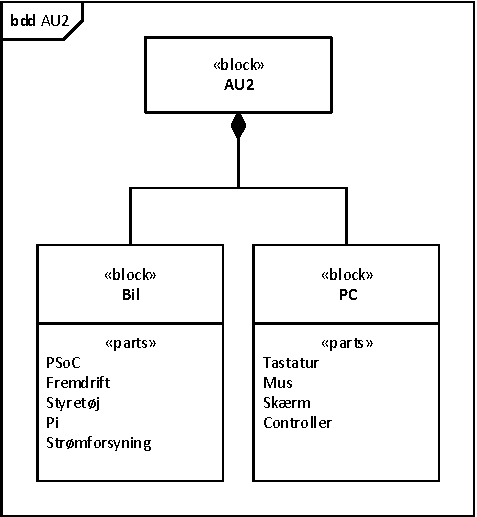
\includegraphics[scale=1]{../fig/diagrammer/bdd_au2.pdf}
\caption{Overordnet BDD for AU2}
\label{fig:bdd_au2}
\end{figure}
På figur \ref{fig:bdd_au2} ses et overordnet BDD for AU2. Det ses at systemet AU2 består af en bil og en PC. Bilen består af en \texttt{PSoC} som er et mikroprocessor-modul der styrer afstandssensorerne. Fremdrift er modulet der sikre bilen fremdrift, herunder motor osv. Styretøj er modulet der har med styretøjet at gøre som gør det muligt for brugeren at dreje med bilen. Pi er en Raspberry-Pi som er en computer der kører et linux program som kører hele komminukationen med PC'en. Strømforsynings-blokken er rimelig selvsigende. PC modulet består af et tastatus, mus, skærm og en Xbox-360 controller. På figur \ref{fig:bdd_bil} ses et udviddet BDD for bilen.  

\begin{figure}[h]
\centering
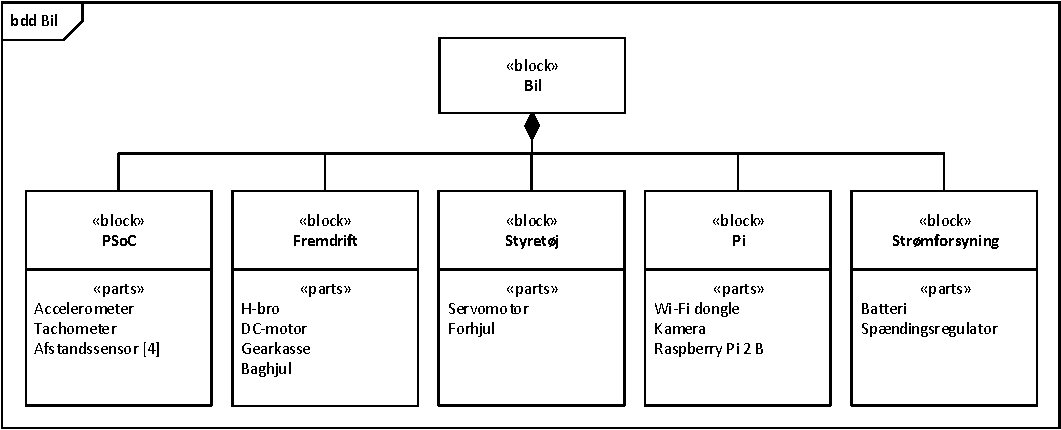
\includegraphics[width=\textwidth]{../fig/diagrammer/bil/bdd_bil.pdf}
\caption{BDD for bil}
\label{fig:bdd_bil}
\end{figure}

På figur \ref{fig:bdd_bil} ses at \texttt{PSoC} består af et Accelerometer til at måle bilens acceleration, et tachometer til at måle bilens hastighed samt fire afstandssensor. Fremdrift består af en H-bro til at styre motorens omdrejningsvinkel, en DC-motor en gearkasse og baghjul. Her er der dog to baghjul og ikke et som angivet i diagrammet. Styretøj består af en servomotor samt forhjul. Pi er bestående en  Raspberry-Pi som er påmonteret med en Wifi-dongle samt et kamera. Strømforsyningen indeholder et batteri samt en spændingsregulator. Spændingsregulatoren er dog implementeret som en switchmode-powersupply.  

\begin{figure}[h]
\centering
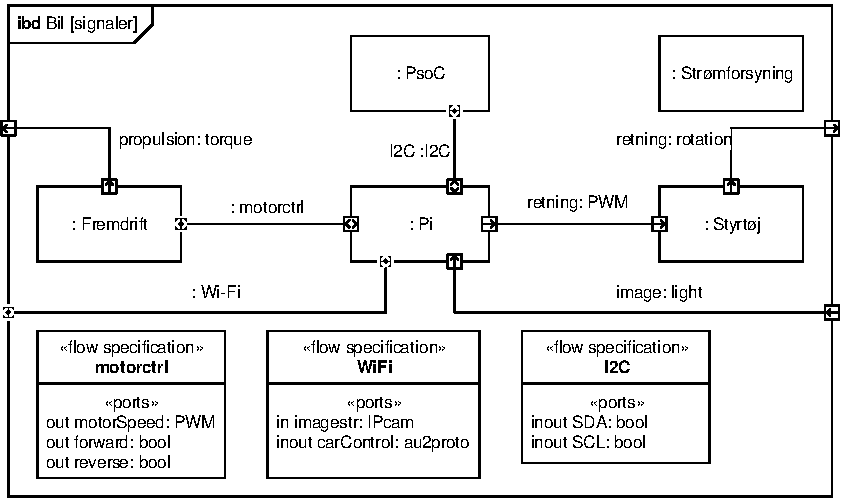
\includegraphics[scale=1]{../fig/diagrammer/bil/ibd_bil.pdf}
\caption{IBD for bil}
\label{fig:ibd_bil}
\end{figure} 

\clearpage